\section{METODOLOGÍA}
%\section[Metodología]{METODOLOGÍA}
%El presente trabajo se basará en el tipo de investigación exploratorio-experimental. 
La presente investigación es de tipo experimental porque se adapta el modelo de conducción autónoma a las vías de doble sentido, la cual es la realidad que se está simulando.

La metodología a usar será ``Cross-industry standard process for data mining'' (CRISP-DM), la cual está diseñada para proyectos de minería de datos y modelos de analíticas. Esta metodología es empleada principalmente por IBM para sus proyectos de analísticas y está integrada en su producto SPSS \citep{Chapman2000CRISPDM1S}.

Esta metodología se compone por 6 fases:

\begin{itemize}[nosep]
    \item \textbf{Comprensión del Negocio:} es la fase de propuestas de objetivos y requisitos del proyecto para convertirlo en una tarea de minería de datos o analíticas.
    \item \textbf{Comprensión de los Datos:} inicia con la recolección de datos y se debe familiarizar con estos, para analizar su calidad y descubrir patrones de utilidad.
    \item \textbf{Preparación de los Datos:} compuesto por todas las tareas de preparación con el fin de construir el dataset final. Estas tareas se realizaran múltiples veces sin orden específico dependiendo de las necesidades del dataset, y pueden ser limpieza de datos, transformaciones y construccones de nuevos atributos.
    \item \textbf{Modelado:} se modelan los datos mediante modelos de aprendizaje automático y técnicas de extracción de la información e inferencia.
    \item \textbf{Evaluación:} se evalúan las capacidades de predicción y ajuste de los modelos sobre los datos, con el fin de elegir el mejor modelo o la mejor combinación de estos.
    \item \textbf{Despliegue:} se aplican los modelos en la vida real para las situaciones que fueron diseñados.
\end{itemize}

\begin{figure}[H]
    \centering
    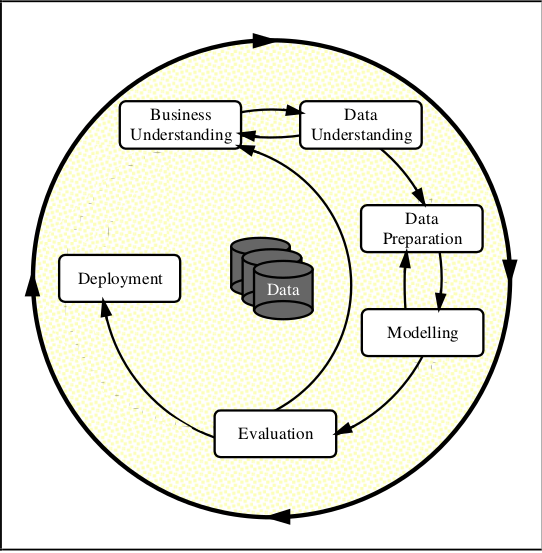
\includegraphics[scale=0.3]{imagenes/crisp}
    \caption[Diagrama CRISP-DM]{Diagrama CRISP-DM\\Fuente: \citep{Wirth00crisp-dm:towards}}
\end{figure}